%% This is an example first chapter.  You should put chapter/appendix that you
%% write into a separate file, and add a line \include{yourfilename} to
%% main.tex, where `yourfilename.tex' is the name of the chapter/appendix file.
%% You can process specific files by typing their names in at the 
%% \files=
%% prompt when you run the file main.tex through LaTeX.
\chapter{The CMS experiment}
The major goal of the CMS detector is to elucidate the EWSB through the discovery of the Higgs boson. However, the CMS is a general purpose detector enabling to perform precision SM measurements as well BSM physics searches at the \TeV scale. The detector goals to meet the requirements of the physics program include good reconstruction and momentum resolution of charged particles, good electromagnetic energy resolution, as well as good di-jet mass and missing energy resolutions. The large number of charged particles per interactions and the additional pileup interactions require a high granularity detector to be able to reconstruct all the individual charged particles.  Furthermore, a bunch spacing of $25$ ns requires a detector with good time resolution to be able to resolve the individual bunch crossings.  

The overall layout of the CMS detector is shown in Figure~\ref{fig:cms}. The detector is composed of several sub-detector layers with a length of $22$ m and a diameter of $15$ m. It has a cylindrical geometry with concentric barrel shaped detectors in the central region and disc shaped detectors in the forward region. The main feature of the CMS detector is a $3.8$ Tesla superconducting solenoid magnet that provides a large bending power. The length of the solenoid is $13$ m and the inner diameter is $6$ m. The inner tracking detectors, electromagnetic, and hadronic calorimeters are located inside the solenoid. The muon detectors are embedded in the steel flux-return yoke of the magnet with sufficient magnetic field to bend the muons inside the muon detectors. The total weight of the CMS detector is $12500$ tonnes.  

\begin{figure}[h]
\centering
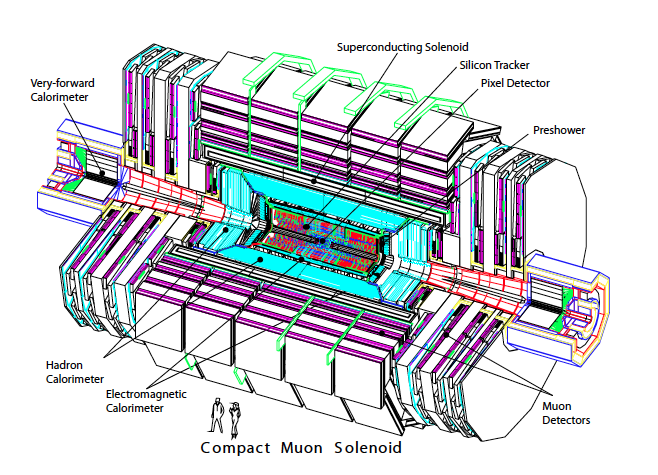
\includegraphics[width=1.0\columnwidth]{figures_chapter3/cms_detector}
\caption{A cutaway diagram of the CMS detector. The labels identify the different sub-detectors and the solenoid.}
\label{fig:cms}
\end{figure}

The CMS uses the right-handed coordinate system. The origin is centered at the nominal collision point, x-axis is in the horizontal plane pointing towards the centre of the LHC tunnel, y-axis points vertically upwards, and the z-axis points along the beam direction toward the Jura mountains. It is convenient to employ the spherical coordinate system. The polar angle  $\theta$ is measured with respect to the positive z-axis and the azimuthal angle $\theta$ is measured from the positive x-axis in the x-y coordinate plane. The pseudorapidity is defined as $\eta = -\ln \tan(\frac{\theta}{2})$.  A useful consequence of this definition is that the difference between the pseudorapidities of two particles is Lorentz invariant with respect to a boost in the beam direction. The separation of two particles is defined by $\Delta R = \sqrt(\Delta \phi^2 + \Delta \eta^2)$. The momentum and energy transverse to the beam direction are denoted $p_{T}$ and $E_{T}$ respectively. The imbalance of the measured transverse energy is defined as the missing energy and denoted by $E_{T}^{miss}$.     

\section{Inner tracking detectors}

The inner tracking system\cite{Karim�ki:368412,addendum} surrounds the interaction point and has a length of $5.8$ m and a diameter of $2.5$ m. The goal of the inner tracking system is to make a precise and efficient measurement of the trajectories of charged particles as well as their momentum. In addition a precise reconstruction of secondary vertices is needed for identification of heavy flavor particle decays. Tau lepton decays are identified by looking for one-prong and three-prong topologies in the inner tracker. A homogenous magnetic field of $4$ Tesla over the full volume of the tracker is provided by the CMS solenoid. 

There are $\Omega(1000)$ particles emerging from the interaction region at the nominal LHC luminosity for every $25$ ns bunch crossing. Therefore a high granular, fast, and radiation hard detector is required. On the other hand this implies a large power density of electronics and the corresponding cabling and cooling systems which increase the amount of material thereby enhancing multiple scattering, photon conversions, and bremsstrahlung.    Silicon technology was chosen given the above considerations. Figure~\ref{fig:tracker} shows a schematic view of the inner tracking system in $r-z$ plane. The inner tracking detector covers a pseudorapidity range of up to $\eta=2.5$ and provides an average $13-17$ measurements per charged particle depending on the $\eta$ region.

\begin{figure}[h]
\centering
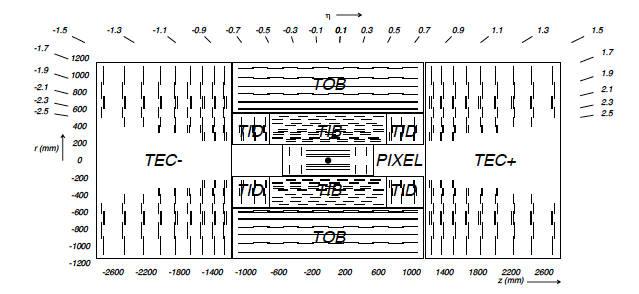
\includegraphics[width=1.0\columnwidth]{figures_chapter3/tracker_layout}
\caption{A schematic view of the CMS tracking system. Silicon pixel and strip detectors are shown. Double lines show back-to-back modules that deliver stereo hits.}
\label{fig:tracker}
\end{figure}

A pixelated detector has to be used close to the interaction region to keep the occupancy levels to less than $1\%$. It consists of three barrel layers and two endcap disks. The barrel layers are located at radii of $4.4$, $7.3$, and $10.2$ cm with a length of $53$ cm. The endcap pixel layers are located at $z=\pm 34.5$ and $z=\pm46.5$ cm covering approximately $6$ to $15$ cm in radial direction. The pixel detector consists of $66$ million pixel elements covering a surface area of approximately of $1$ m$^2$. The pixel element size is $100\times150$ $\mu$m$^2$ providing similar track resolution in both $r-\phi$ and $r-z$ directions. Each pixel is a $p-n$ semiconductor junction. When a charged particle passes through the depletion region of the junction an electron-hole pairs are created and subsequently collected by the readout electronics. The Lorentz drift in the CMS magnetic field leads to charge spreading of the collected signal charge between adjacent pixels. Using an analog pulse height read out the charge sharing allows to reduce a single hit spatial resolution to $15-20$ $\mu$m.  

The outer tracker is occupied by a silicon strip tracker allowing two-dimensional measurements. Majority of the strips are oriented perpendicular to the $\phi$ direction, parallel to the beam direction in the barrel region and aligned radially in the endcap region. The tracker Inner Barrel (TIB) is located in the barrel region and extends from $20$ cm to $55$ cm in the radial direction. There are $6$ additional layers with an outer radius of $116$ composing the Tracker Outer Barrel (TOB) and extending in $|z|$ to $118$ cm. The Tracker Disk (TID) consists of $3$ layers located from $|z|$ of $80$ and $90$ cm. The Tracker EndCap (TEC) has nine layers and covers the region between $|z|$ of  $124$ and $282$ cm. These radial strips provide up to  $9$ $\phi$ measurements for each trajectory. The silicon strip tracker has a total of $9.3$ million strips and covers a surface area of $198$ m$^2$. The strip pitch varies between $80$ and $184$ $\mu$m depending on the region of interest. In addition, there is a second strip module mounted back-to-back with a stereo angle of $100$ mrad in in the first layers. This allows a measurement of the $z$ and $r$ coordinates in the barrel and disks respectively. The corresponding resolution in z co-coordinate is $230$ to $530$ $\mu$m in TIB and TOB.  

\section{Electromagnetic calorimeter}



\section{Hadronic calorimeter}

\subsection{LS1 Upgrades}

\section{Muon Detectors}

\section{Triggering and Data Acquisition}
    



